\documentclass[conference]{IEEEtran}

\usepackage{listings}
\usepackage{cite}
\usepackage{amsmath,amssymb,amsfonts}
\usepackage{algorithm}
\usepackage{algorithmic}
\usepackage{graphicx}
\usepackage{textcomp}
\usepackage{xcolor}

% Define OCaml language for listings
\lstdefinelanguage{OCaml}{
    keywords={let, in, fun, if, then, else, match, with, type, val, module, open},
    sensitive=true,
    comment=[l]{//},
    morecomment=[s]{(*}{*)},
    string=[b]{"},
    morestring=[b]{"},
}

% Set the style for OCaml code
\lstset{
    language=OCaml,
    basicstyle=\ttfamily\small, % Use small font size for better fit
    keywordstyle=\color{blue},
    commentstyle=\color{green},
    stringstyle=\color{red},
    numbers=left, % Position of line numbers
    numberstyle=\tiny\color{gray}, % Style of line numbers
    stepnumber=1,
    numbersep=5pt,
    frame=none, % Turn off the frame around the code
    tabsize=2,
    showstringspaces=false,
    breaklines=true, % Allow line breaking
    linewidth=\columnwidth, % Set the width to the column width
    firstnumber=1, % Start numbering from 1
}
\def\BibTeX{{\rm B\kern-.05em{\sc i\kern-.025em b}\kern-.08em
    T\kern-.1667em\lower.7ex\hbox{E}\kern-.125emX}}
\begin{document}

\title{Ray Tracing In Functional Programming Language\\

}

\author{\IEEEauthorblockN{Dr. Babul Prasad Tewari}
\IEEEauthorblockA{\textit{Department of} \\
\textit{ Computer Science and Engineering}\\
\textit{GKCIET}\\
Malda, India \\
babul@gkciet.ac.in}
\and
\IEEEauthorblockN{Aditya Raj}
\IEEEauthorblockA{\textit{Department of} \\
\textit{ Computer Science and Engineering}\\
\textit{GKCIET}\\
Malda, India \\
induaditya214@gmail.com}
\and
\IEEEauthorblockN{3\textsuperscript{rd} Given Name Surname}
\IEEEauthorblockA{\textit{dept. name of organization (of Aff.)} \\
\textit{name of organization (of Aff.)}\\
City, Country \\
email address or ORCID}
}

\maketitle

\begin{abstract}
to do
\end{abstract}

\begin{IEEEkeywords}
ray tracing, three-dimensional graphics, functional programming.
\end{IEEEkeywords}

\section{Introduction}

There are two approaches to rendering a three-dimensional scene: object-order rendering and image-order rendering. \cite{peter}

Object-order rendering involves iterating over each object and figuring out which set of pixels it maps to and coloring those pixels.
In image-order rendering, for each pixel, the nearest visible object is found, and that pixel is colored using the given shading model. 
The former is classified into rasterization algorithms (or projective algorithms), and the latter is termed the ray tracing algorithm (image-space algorithm). Same effects, like reflections and shadows, are easy to implement in ray tracing compared to rasterization\cite{kevin}.

In ray tracing, image synthesis happens by shooting rays that go through the projection plane, and the nearest intersection with an object is found. If the object is reflective, rays bounce off it and hit other objects, which also influences color according to the shading model\cite{kevin}. In the current implementation\cite{mycode}, we have utilized the simplest shading model called Phong shading\cite{peter} and used the simplest three-dimensional geometrical object, a sphere, to illustrate ray tracing in the functional programming paradigm. To this end, we decided to use OCaml for its strong support for functional programming and its mechanisms to write imperative code as well, which will enable us to demonstrate alternative ways in the same programming language.

\section{Architecture}
We defined following functionalities for our ray tracer as illustrated through figures.

\begin{figure}[htbp]
  \centerline{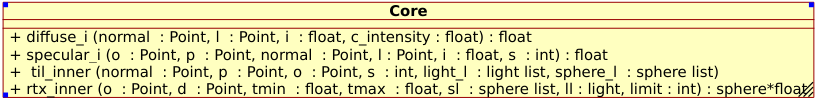
\includegraphics[width=0.38\textwidth]{./figs/corediagram.png}}
  \caption{Core functions}
\end{figure}

\begin{figure}[htbp]
  \centerline{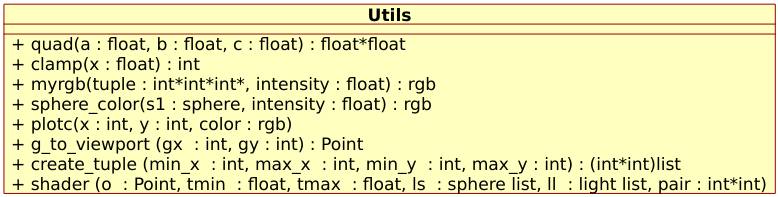
\includegraphics[width=0.48\textwidth]{./figs/utilsdiagram.png}}
  \caption{Utility functions}
\end{figure}

\begin{figure}[htbp]
  \centerline{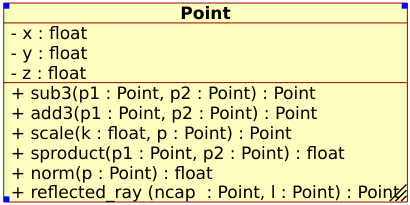
\includegraphics[width=0.38\textwidth]{./figs/pointdiagram.png}}
  \caption{Point type}
\end{figure}

\begin{figure}[htbp]
  \centerline{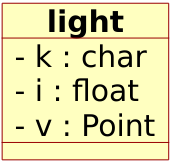
\includegraphics[width=0.1\textwidth]{./figs/lightdigram.png}}
  \caption{Light type}
\end{figure}

\begin{figure}[htbp]
  \centerline{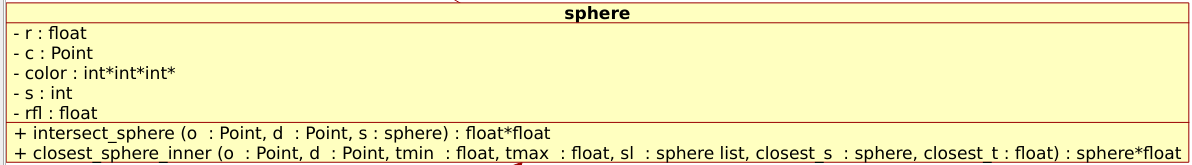
\includegraphics[width=0.58\textwidth]{./figs/spherediagram.png}}
  \caption{Sphere type}
\end{figure}

\section{Coordinate System}

In the OCaml standard graphics library, the origin of the drawing window is situated at the bottom left corner. For convenience, we want it in the middle of the window. Thus, so we wrote wrapper function \textit{plotc}.

This function translates the origin to the middle of the graphics window.

\section{Colors}

We use the additive color model (RGB model), where each color channel is represented by an 8-bit positive integer. Therefore, the range is $[0,255]$. We can treat the triplet of RGB values as a vector. Adding two colors together yields a new color, and multiplying a color by a scalar increases its brightness, i.e.,

$$k (r, g, b) = (kr, kg, kb)$$

There is a chance that any channel value may go out of the range $[0,255]$ while manipulating colors. We can handle this as follows:

Suppose there is a channel value $x$:
\begin{itemize}
    \item If $x > 255$, then we set $x = 255$.
    \item If $x < 0$, then we set $x = 0$.
\end{itemize}

This process is called \textit{clamping}.

\section{Scene}

The scene is simply a set of objects that we want to render on the screen.

To represent objects in a scene, we need to use a 3D coordinate system that employs real numbers to represent continuous values, which are then mapped to a discrete 2D graphics window while drawing.

The viewing position from which we look at the scene is called the \textbf{camera position}. We assume that the camera is fixed and occupies a single point in space, which will often be the origin $O(0,0,0)$.

The \textit{camera orientation}\cite{peter} is the direction in which the camera points, or from where rays enter the camera. We will assume the camera orientation to be $Z_+$, the positive z-axis.

The frame has dimensions $V_w$ and $V_h$ and is frontal to the camera (perpendicular to the camera orientation, irrespective of camera position, in our case perpendicular to $Z_+$) and at a distance $d$ away from the camera. Technically, this is called the \textit{viewport}\cite{peter}.

The angle visible from the camera is called the \textit{field of view} (FOV).\cite{peter} It depends on the distance $d$ from the camera to the viewport and the dimensions of the viewport $V_w$ and $V_h$.

In our case, we assume 

$$V_w = V_h = d = 1 \implies FOV \approx 53^\circ$$

We will represent the coordinates of the viewport as $(V_x,V_y)$ in worldly units and the graphics window as $(G_x,G_y)$ in pixels. Thus, the conversion is given by:

$$V_x = G_x \times \frac{V_w}{G_w}$$

$$V_y = G_y \times \frac{V_h}{G_h}$$

where $G_w$ and $G_h$ are the maximum width and height of the graphics window, respectively.

However, we know that the viewport is in 3D space, so it also has $V_z = d$ for every point on this viewport (in mathematical terms, called the \textit{projection plane}). \\
Thus, for every pixel $(G_x, G_y)$ on the graphics window, we can calculate the corresponding $(V_x, V_y, V_z)$ of the viewport.

\section{Phong Shading Model}

\begin{algorithm}
    \caption{Ray Tracing Algorithm}
    \begin{algorithmic}[1]
        \STATE Initialize scene with objects and lights
        \STATE Set canvas resolution (width, height)
        \STATE For each pixel (x, y) in the canvas:
            \STATE \quad Generate ray from camera through pixel (x, y)
            \STATE \quad Initialize color to background color
            \STATE \quad Initialize closest intersection distance to infinity
            \STATE \quad For each object in the scene:
                \STATE \quad \quad If ray intersects object:
                    \STATE \quad \quad \quad Calculate intersection point
                    \STATE \quad \quad \quad Calculate normal at intersection point
                    \STATE \quad \quad \quad Calculate distance to intersection
                    \STATE \quad \quad \quad If distance is less than closest intersection distance:
                        \STATE \quad \quad \quad \quad Update closest intersection distance
                        \STATE \quad \quad \quad \quad Calculate color at intersection point
                        \STATE \quad \quad \quad \quad Update color based on lighting
            \STATE \quad Set pixel color to calculated color
        \STATE Render the image
    \end{algorithmic}
\end{algorithm}
 
\subsection{Diffuse Reflections}

Now, we will calculate the illumination of a point by both a point source and a directional source through diffuse reflection.

Consider a point $ P $ in the scene, with $ \vec{N} $ representing the normal vector at $ P $ and $ \vec{L} $ as the directional vector of the light source. For directional light, $ \vec{L} $ is provided. However, for a point light source, we need to compute $ \vec{L} $ based on the position of the light source and the coordinates of point $ P $. Let $ l $ denote the width of the light (which is proportional to its intensity) and $ x $ denote the distance over which the light spreads. The line $ RS $ is perpendicular to $ \vec{L} $, and $ Q $ is the point of intersection.

The ratio $ \frac{l}{x} $ represents the drop in intensity after the light reflects off the surface. For instance, if the light is perpendicular to point $ P $ on the surface, then $ \frac{l}{x} = 1 $.

\begin{figure}[htbp]
    \centerline{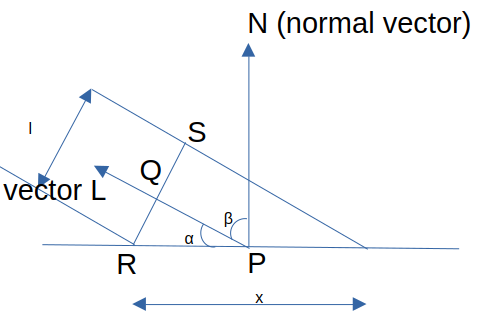
\includegraphics[width=0.38\textwidth]{./figs/intensity.png}}
    \caption{Intensity after diffuse reflection}
\end{figure}

Consider the right triangle $ \triangle PQR $. It is evident that 

$$\angle PRQ = \beta$$

Using the definition of cosine in a right triangle, we have:

$$\cos \beta = \frac{l/2}{x/2} = \frac{l}{x}$$

We also know that the dot product of the vectors can be expressed as:

$$\langle \vec{L}, \vec{N} \rangle = \|\vec{L}\| \|\vec{N}\| \cos \beta.$$

Thus, we can rewrite $ \cos \beta $ as:

$$\cos \beta = \frac{\langle \vec{L}, \vec{N} \rangle}{\|\vec{L}\| \|\vec{N}\|}.$$

If $ \beta > 90^\circ $, the point is illuminated from the backside of the surface, and in this case, we treat the intensity as zero.

To obtain the intensity after reflection, we multiply the intensity of the light by the factor $ \cos \beta $.

In a scene, a single point can be illuminated by multiple light sources, which may vary in type. We simply sum the intensities of all the light sources that reach the point and then multiply the total intensity by the color of the point, which effectively adjusts the brightness.

Mathematically, this can be expressed as:
\begin{equation}
    I_{\text{diffused}} = \sum I_i \frac{\langle \vec{L_i}, \vec{N} \rangle}{\|\vec{L_i}\| \|\vec{N}\|}
    \label{diffuse}
\end{equation}
    

where\\
- $ I_{\text{diffused}} $ is the intensity due to diffuse reflection,\\
- $ I_i $ is the intensity of the $ i^{\text{th}} $ light source, which can be either a point source or a directional light,\\
- $ \vec{L_i} $ is the directional vector of the $ i^{\text{th}} $ light source.




\subsection{Specular reflection}

\begin{figure}[htbp]
    \centerline{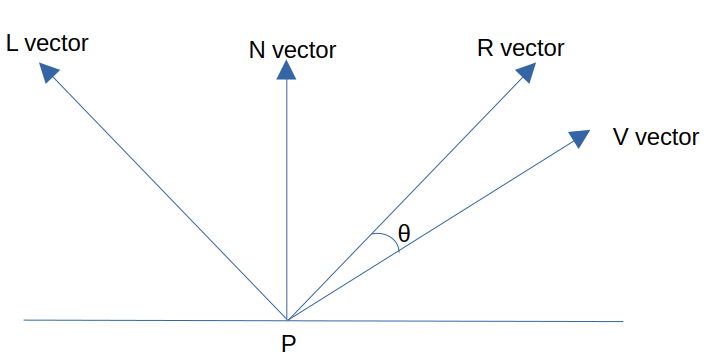
\includegraphics[width=0.38\textwidth]{./figs/intensityspecular.png}}
    \caption{Intensity after specular reflection}

\end{figure}
To model it, we use the simple fact that the angle made by the incident ray with the normal is equal to the angle made by the reflected ray with the normal .

Here\\
- $\vec{L}$ is the directional vector of light pointing from point $P$ on the surface to the point light source.\\
- $\vec{R}$ is the reflected light, which makes the same angle with $\vec{N}$ as $\vec{L}$.\\
- $\vec{V}$ is the view vector from point $P$ on the surface to the camera.\\
- $\vec{N}$ is the normal vector.\\

First, we express $\vec{R}$ in terms of $\vec{L}$ and $\vec{N}$.
We know that $\vec{L}$ can be split into two components: one parallel to $\vec{N}$ and another perpendicular to it.
$$\vec{L_{\| \vec{N}}} = \langle \vec{L}, \hat{N} \rangle \hat{N}$$

Since 

$$\vec{L_{\| \vec{N}}} + \vec{L_{\perp \vec{N}}} = \vec{L}$$

we have
$$\implies \vec{L_{\perp \vec{N}}} = \vec{L} - \langle \vec{L}, \hat{N} \rangle \hat{N}$$

Thus, we can express $\vec{R}$ as:
$$\vec{R} = \vec{L_{\| \vec{N}}} - \vec{L_{\perp \vec{N}}}$$
$$\implies \vec{R} = 2 \langle \vec{L}, \hat{N} \rangle \hat{N} - \vec{L}$$

Now we determine the intensity due to specular reflection. For $\theta = 0$, the reflected vector and the view vector align, so brightness is at its maximum. If $\theta = 90^\circ$, no component of the reflected ray is in the direction of the view vector, so brightness is zero in this case.

For $0 \leq \theta \leq 90^\circ$, we use $\cos \theta$ to model brightness. We define $s$ to vary the shininess of different objects.

Then, the final expression for brightness due to specular reflection is:

\begin{equation}
    I_{\text{specular}} = \sum I_i (\cos \theta)^s = \sum I_i \left( \frac{\langle \vec{R_i}, \vec{V_i} \rangle}{\|\vec{R_i}\| \|\vec{V_i}\|} \right)^s
    \label{specular}
\end{equation}

Note that if $\theta > 90^\circ$, we might get a negative total intensity, which doesn't make sense. In those cases, we set the term to zero as before.

Combining both diffuse and specular brightness, along with ambient light, we get:

\begin{equation}
    {I_{\text{total}} = I_a + \sum I_i \left[ \frac{\langle \vec{L_i}, \vec{N} \rangle}{\|\vec{L}_i\| \|\vec{N}\|} + \left( \frac{\langle \vec{R_i}, \vec{V} \rangle}{\|\vec{R_i}\| \|\vec{V}\|} \right)^s \right]}
    \label{combined}
\end{equation}

Here\\
- $I_{\text{total}}$ is the total intensity at the point.\\
- $I_a$ is the intensity of ambient light.\\
- $I_i$ is the intensity of the $i$-th light, which could be a point source or directional.\\
- $\vec{L_i}$ is the incident vector of the $i$-th light.\\
- $\vec{R_i}$ is the reflected vector of the $i$-th light.\\
- $\vec{N}$ is the normal vector at the point.\\
- $\vec{V}$ is the view vector at the point.\\

\subsection{Shadows }

A shadow is the obstruction of light by one or more objects at a point.

What this means for us is that we need to check if a particular light source, such as a point source or directional light, intersects any other object in the scene before reaching the point for which we are calculating illumination due to that light. If that intersection occurs, then we do not include that light's intensity in the calculation of the total intensity; otherwise, we do.

In order to do that, we shoot a ray from the point of interest (for which we want to know whether it is shadowed) in the direction of the light source.

That ray is represented as 

$$\vec{R} = P + t \vec{L}$$

Here

- $P$ is the point of interest.
- $\vec{L}$ is the ray of light from $P$ toward the light source.
- $t$ is the parameter. For a point source, $t \in [0^+, 1]$ (at $t = 1$, we reach the light source itself), and for directional light, $t \in [0^+, \infty)$. We know that a point on a sphere will definitely intersect itself, so practically we take $0.0001$ instead of $0^+$. (We tried using $\epsilon_{\text{float}}$ and the results were not visually appealing, so to speak.)

Next, we find the closest intersection of the sphere with the ray in the suitable range. If a sphere exists, then only ambient light illuminates that point; otherwise, both specular and diffuse reflections also occur.

\subsection{Mirror Reflection}

After a ray from a camera intersects at a point on an object, we find the reflected ray at that point (including its color) and then shoot a reflected ray to determine if it intersects another object and calculate the resulting color. We can do this as many times as we like (but usually, after three reflections, we observe diminishing returns per computation). Eventually, we take a weighted sum of all the colors, utilizing the `rfl` property of spheres.

\section{Total Intensity of Light}

Here, we combine all the effects, such as different kinds of reflection, into a single function, except for mirror reflection, which is handled through the ray tracing code itself.


\begin{lstlisting}
    let rec til_inner normal p o s light_l sphere_l intensity = 
  match light_l with 
  {k;i;v}::t -> 
    let c_intensity = ref 0. in
    let tmax = ref 0. in 
    if k = 'a' then c_intensity := i +. !c_intensity 
    else 
      begin
        let l = ref {x=0.;y=0.;z=0.} in
        (if k = 'p' then
            (l := (sub3 (bare v) p); 
            tmax := 1.)
          else  
           (l := bare v;
           tmax := infinity));
          let shadow_s,_ = closest_sphere p !l 0.0001 !tmax sphere_l in 
          match shadow_s with 
          Some ss -> ()
          |_ -> 
            let unitnormal = scale (1. /.(norm normal)) normal in 
          c_intensity := specular_i o p unitnormal !l i s !c_intensity;
          c_intensity := diffuse_i normal !l i !c_intensity
      end;
    til_inner normal p o s t sphere_l (intensity +. !c_intensity)
  | _ -> intensity;;

let til normal p o s light_l sphere_l = til_inner normal p o s light_l sphere_l 0.;;
\end{lstlisting} 

\section{Ray tracing code}

\begin{lstlisting}
let rec rtx_inner o d tmin tmax sl ll limit =
  let objintensity = ref 0. in 
  let otherintensity = ref 0. in  
  let s, t = closest_sphere o d tmin tmax sl in 
  begin
    match s, t with 
    Some sphere, Some t_parameter ->
      let p = add3 o (scale t_parameter d) in 
      let normal = sub3 p sphere.c in
      objintensity := til normal p o sphere.s ll sl;
      if sphere.rfl > 0. && limit > 0 then
        begin
          let reflected = reflected_ray (scale (1. /. norm normal) normal) (scale (- 1.) d) in 
          otherintensity := extract (rtx_inner p reflected 0.001 infinity sl ll (limit-1));
          objintensity := !objintensity *. (1. -. sphere.rfl) +. sphere.rfl *. !otherintensity;
        end
    | _, _ -> ()
  end; 
  s, !objintensity;;

let rtx o d tmin tmax sl ll = sphere_color (rtx_inner o d tmin tmax sl ll 3)
\end{lstlisting}

Now there two ways to start the ray tracing: 
In functional style:

\begin{lstlisting}
let create_tuple min_x max_x min_y max_y =
  let rec range start stop a = 
      if start > stop then a
      else range (start + 1) stop (start::a)
  in 
  let list_x = range min_x max_x [] in
  let list_y = range min_y max_y [] in 
  let a l x = List.map  (fun y -> (x, y))  l
  in
  List.flatten (
      List.map  (a list_y)  list_x
      )

let shader o tmin tmax ls ll (x, y) = 
    let v = g_to_viewport x y in
            let d = sub3 v o in
            let color = rtx o d tmin tmax ls ll in 
            plotc x y color

let coordinates = create_tuple (-gw/2) (gw/2) (-gh/2) (gh/2) in 
    List.iter (shader o 1. infinity ls ll ) coordinates
\end{lstlisting}

And in imperative style:

\begin{lstlisting}
for y = - gh/2 to gh/2 do 
  for x = - gw/2 to gw/2 do 
      let v = g_to_viewport x y in
      let d = sub3 v o in
      let color = rtx o d 1. infinity ls ll in 
      plotc x y color
  done;
done
\end{lstlisting}
\begin{thebibliography}{00}
\bibitem{b1} A. Glassner, ``An Introduction to Ray Tracing,'' Morgan Kaufmann, 1989.

\bibitem{ericm} E. Lengyel, ``Mathematics for 3D game programming and computer graphics,'' Cengage Course Technology PTR, 2019.

\bibitem{b3} R. Hartley, A. Zisserman, ``Multiple view geometry in computer vision,'' Cambridge University Press, 2004.

\bibitem{kevin} K. Suffern, ``Ray tracing from the ground up,'' CRC Press, 2007.

\bibitem{b5} P. Shirley, R. K. Moreley, ``Realistic ray tracing,'' A K Peters Ltd, 2003.

\bibitem{ericr} E. Lengyel, ``Foundations of game engine development volume 2: Rendering,'' Terathon Software LLC, 2019.

\bibitem{peter} S. Marschner, P. Shirley, ``Fundamentals of computer graphics,'' CRC Press, 2016.

\bibitem{b8} S. J. Gortler, ``Foundations of 3D computer graphics,'' MIT Press, 2012.

\bibitem{b9} M. Ashikmin, P. Shirley, ``An anisotropic Phong light reflection model,'' Technical Report UUCS-00-014, Computer Science Department, University of Utah, 2000.

\bibitem{b10} J. F. Blinn, ``Models of light reflection for computer synthesized pictures,'' Proceedings of SIGGRAPH 77, Computer Graphics, Vol. 11, No. 2, pp. 192–198, 1977.

\bibitem{b11} M. F. Cohen, J. R. Wallace, ``Radiosity and realistic image synthesis,'' Academic Press, San Diego, CA, 1993.

\bibitem{b12} R. L. Cook, K. E. Torrance, ``A reflection model for computer graphics,'' ACM Transactions on Graphics, Vol. 1, No. 1, pp. 7–24, 1982.
\bibitem{cs1} R. L. McFall,and C. A. Cusack , Ray tracing as an object-oriented example for CS 1, The Journal of Computing Sciences in Colleges, 2010, pp.77--84.

\bibitem{pbrt} M. Pharr and G. Humphreys, ``Physically Based Rendering: From Theory to Implementation,'' Morgan Kaufman, 2004.


\bibitem{mycode} A. Raj, ``Very basic ray tracer,'' 2025, gitHub repository. [Online]. Available: https://github.com/induaditya3/computer\_graphics\_ocaml/\\tree/main/ray\_tracer


\bibitem{b16} T. Whitted, ``An improved illumination model for shaded display,'' Communications of the ACM 23, June 1980.

\bibitem{b17} J. F. Hughes, A. van Dam, M. McGuire, D. F. Sklar, J. D. Foley, S. K. Feiner, K. Akeley, ``Computer graphics: Principles and Practice,'' Addison-Wesley, 2013.
\end{thebibliography}

\end{document}
